% Set scale of images so that both have the same scale.
\sbox0{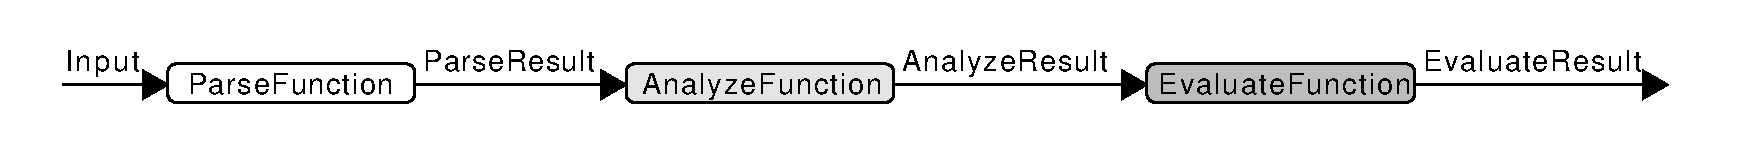
\includegraphics{unit-flow}}
\makeatletter
\Gscale@div\imgscale\textwidth{\wd0}
\makeatother
%
\section{Function Composition}
\label{sec:function-comp}
\begin{figure}[t]
  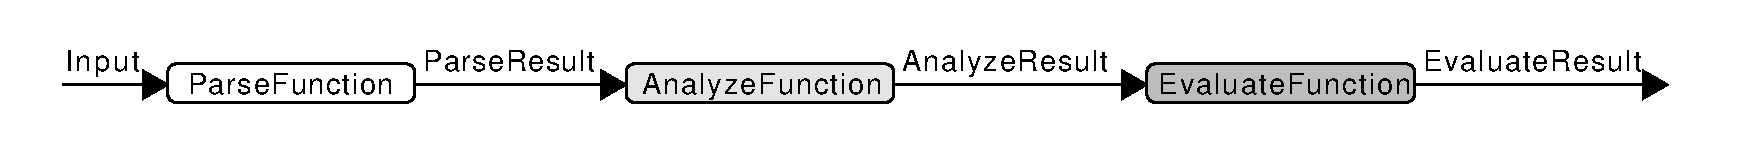
\includegraphics[scale=\imgscale]{unit-flow}
  \includegraphics[scale=\imgscale]{unit-flow-no-analyze}
  \caption{Example composition of execution steps. The top shows the
    execution model of a language with static analysis,
    the bottom shows one without static analysis. }
  \label{fig:unit-flow}
\end{figure}

There was a need for a more fine-grained and flexible way of defining commands
for those that deal with the execution model as described in
\cref{cha:background}. This is because the specific
execution steps that are needed for the evaluation of a program in one language
can differ from those of other languages. For example, some languages
have no analysis stage, whereas some do. The \texttt{LanguageCommand}, as
explained in the previous section, should thus create different
commands depending on whether the loaded language has an
analysis step. See \cref{fig:unit-flow} for a schematic example.

To accommodate for this, commands dealing with the execution model are
built by composing functions using a \texttt{CommandBuilder}, a class
following the builder pattern. In this context, a function represents a
step in the execution model, whereas the composition represents the
execution model as a whole. The builder has methods for composing
functions and a method for building a command like the one described
in the previous section out of the composition. A UML diagram is shown
in \cref{fig:uml-function-comp}.

\begin{figure}[b]
  \centering
  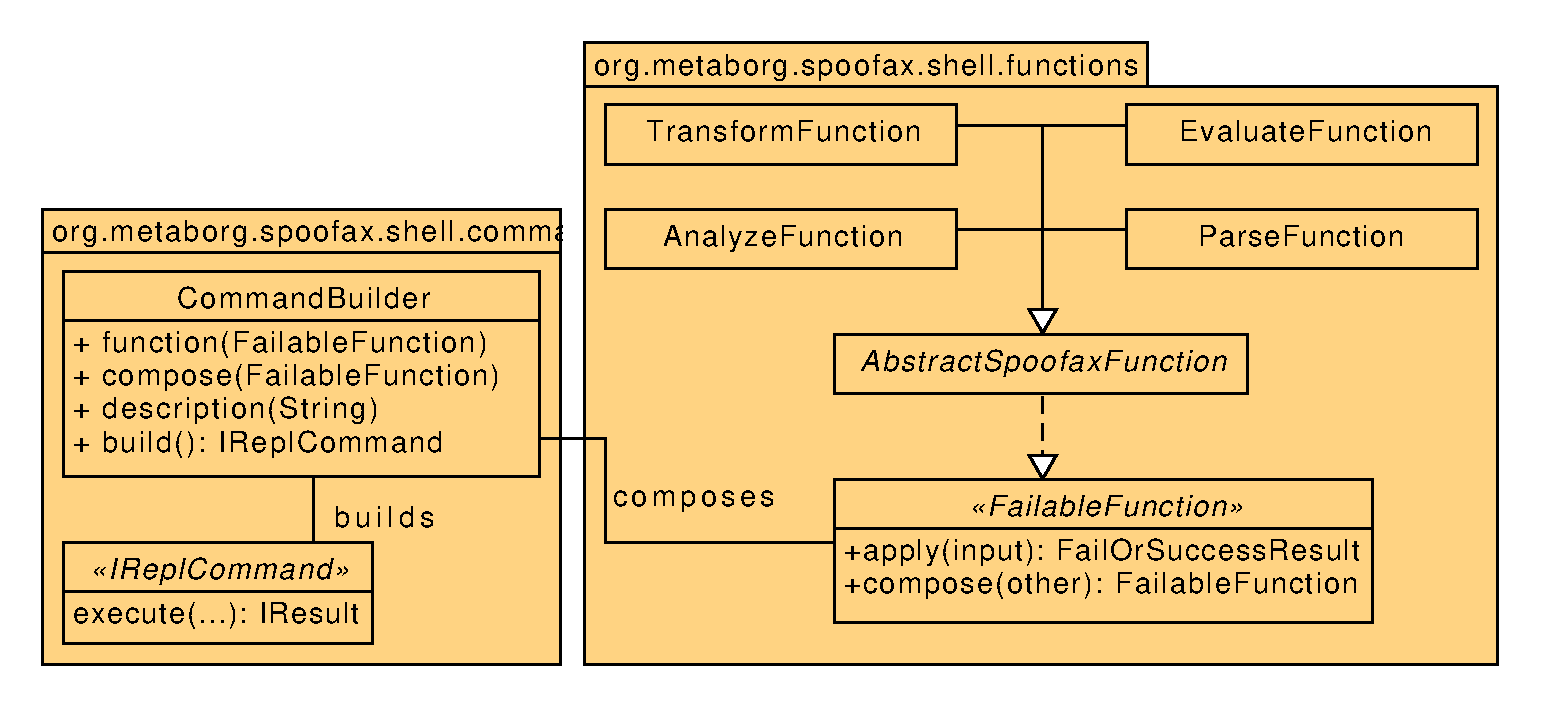
\includegraphics[width=0.8\textwidth]{uml-function-comp}
  \caption{UML of the \texttt{CommandBuilder} and function composition
    interfaces.}
  \label{fig:uml-function-comp}
\end{figure}

This design decision brings several benefits:

\begin{enumerate}
\item It is a direct mapping from the problem domain: functions
  represent execution steps and their composition represents the
  execution model.
\item The functions are reusable, since each function only assumes
  the types of its input and output.
\item It allows for composing and defining commands at runtime.
\end{enumerate}

One problem remains in this design, which is how to handle failures that occur
somewhere in the execution pipeline. For example, analysis should not be
done when parsing has failed. Using Java's exceptions to solve this problem
is not desirable, as one would like to treat failures as any other result of an
execution step. The solution to this problem is to apply monadic composition, as
opposed to regular function composition.

\subsection{Monadic composition}
\label{sec:monadic-composition}
The function composition model takes inspiration from the \texttt{Either}
data type that is known to many functional languages such as
Haskell. It is a data type that represents two alternatives, for
example \textit{either} a success or a failure. As any step in the
execution model of the REPL can result in either a failure (for
example a syntax error) or a success, this data type is a good
candidate for solving the problem of intermediate errors.

The \texttt{Either} type is used as follows: Any individual function in the
execution model returns an \texttt{Either} type, representing the
alternatives of success or failure. When a function is composed with
another function, the latter function is only executed when the former
function returns an \texttt{Either} representing a successful
result. Otherwise, the latter function is not
executed at all and the same \texttt{Either} is returned instead, thereby
propagating the cause of the failure to the end of the pipeline whilst
discarding any other functions further down this execution pipeline.
This kind of function composition is an example of what is known as \textit{monadic
  composition}\footnote{Monads are a more abstract concept than just
  this specific case. In fact, the \texttt{Either} data type is just one
  type of monad.}.

The \texttt{Either} data type has been adopted in the design of the REPL as
a class named \texttt{FailOrSuccessResult}. The class is more specific to
the domain of the execution model of the REPL. It implements the
\texttt{IResult} interface just like any other result class, thereby
allowing it to be treated in the same way generically. The functions
representing the execution steps bear the name \texttt{FailableFunction},
and contain a method for composing it with another
\texttt{FailableFunction}.

%%% Local Variables:
%%% TeX-master: "../main"
%%% End:
